En esta sección del apéndice se muestran distintas modificaciones aplicadas a QAOA sobre algunos de los problemas tratados en el TFG\@.

\section{Camino más corto en grafo de 4 nodos\label{sec:8-primer}}

Partiendo de la solución del artículo\cite{multi-objective_routing_optimization} descrita en la \textit{sección~\ref{sec:5-primer-paper-resultados-qiskit}}, se ha realizado una modificación a la formulación del problema con el fin de obtener un mejor resultado.

Esta modificación ha consistido en añadir una restricción a la función de coste, que especifique que solo se puede acceder al último nodo por una de las aristas que lleguen a este.

\begin{align}\label{eq:5-primer-restriccion_extra}
  X_{13} + X_{23} = 1
\end{align}

La intención con este caso es que, al haber una restricción más, los caminos que rompan dicha restricción tengan un coste aún más elevado.
Así los resultados deberían ser mejores, al filtrar de manera más agresiva ciertos caminos incongruentes.

\begin{table}[Resultados QAOA {--} artículo de Urgelles \textit{et al.} (2022) {--} restricción extra]{tab:5-primer-restriccion_extra-aer_estadisticas}{Resultados de la ejecución de QAOA añadiendo la restricción de la \textit{fórmula~\ref{eq:5-primer-restriccion_extra}}}
  \centering
  \begin{tabular}{|c|r|r|}
    \hline
    \textbf{nº Capas} & \textbf{NA/TE} & \textbf{MM/TE} \\ \hline
    p = 1 & 93.8\% & 37.83\% \\ \hline
    p = 2 & 64.6\% & 26.16\% \\ \hline
    p = 3 & 84.8\% & 27.82\% \\ \hline
    p = 4 & 56.0\% & 23.47\% \\ \hline
    p = 5 & 88.1\% & 46.40\% \\ \hline
    p = 6 & 88.1\% & 21.83\% \\ \hline
  \end{tabular}
\end{table}

Los resultados (\textit{tabla~\ref{tab:5-primer-restriccion_extra-aer_estadisticas}}) presentan una ligera mejora con respecto a los presentes en la \textit{tabla~\ref{tab:5-primer-paper-aer_estadisticas}}, tanto para la estadística \textbf{NA/TE} como para \textbf{MM/TE}.

La función gamma resultante (\textit{fig.~\ref{fig:5-primer_grafo/con_restriccion_extra/primer_restr_aer_gamma_fun}}) toma, en comparación con la original (\textit{fig.~\ref{fig:5-primer_grafo/sin_restriccion_extra/primer_paper_p_27_gamma_fun}}), unos valores elevados.
Se distingue un incremento en la diferencia entre los mínimos globales y los mínimos locales (no globales).

\begin{figure}[Resultados QAOA {--} artículo de Fan \textit{et al.} (2023) {--} función gamma con restricción extra]{fig:5-primer_grafo/con_restriccion_extra/primer_restr_aer_gamma_fun}{Función gamma de \textit{execute\_circuit()} (con $\beta = 1.0$ y variando $\gamma$). Con restricción extra}
  \centering
  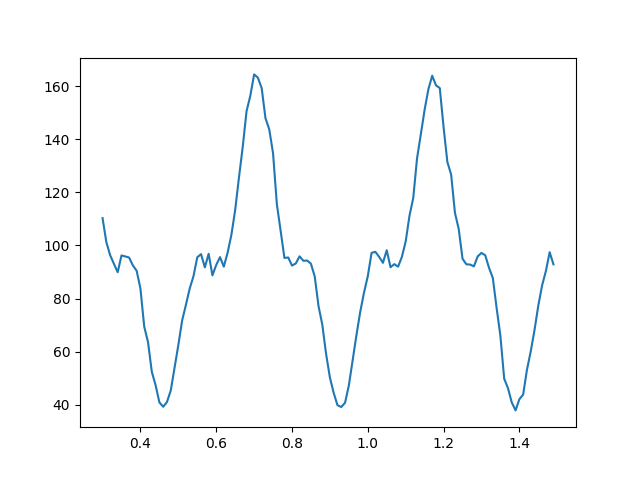
\includegraphics[scale=0.5]{primer-grafo/con_restriccion_extra/primer_restr_aer_gamma_fun.png}
\end{figure}

En definitiva, aunque sí se obtienen unos resultados con un mayor índice de la métrica \textbf{NA/TE} que los de la \textit{sección~\ref{sec:5-primer-paper-resultados-qiskit}}, no es una mejora lo suficientemente pronunciada como para incluir este caso en la sección de resultados.


\section{Camino más corto para estudiar la variación con el número de capas\label{sec:8-zhiqiang}}

\subsection{Camino más corto omitir variabilidad en puertas $Rz$}

Como primera modificación se ha omitido la variable $\gamma$ de los operadores $Rz$, haciendo así que se cometa una imprecisión igual a la del artículo publicado por Urgelles \textit{et al.} (2022)\cite{multi-objective_routing_optimization}.

\begin{table}[Resultados QAOA {--} artículo de Fan \textit{et al.} (2023) {--} puertas $Rz$ constantes]{tab:5-zhiqiang-aer_estadisticas}{Ejecución de QAOA del camino más corto en grafo de la \textit{fig.~\ref{fig:4-zhiqiang_grafo}}}
  \centering
  \begin{tabular}{|c|r|r|}
    \hline
    \textbf{nº Capas} & \textbf{NA/TE} & \textbf{MM/TE} \\ \hline
    p = 1 &  0.6\% &  5.9\% \\ \hline
    p = 2 & 30.7\% & 16.9\% \\ \hline
    p = 3 & 93.8\% & 26.0\% \\ \hline
    p = 4 & 66.9\% & 39.4\% \\ \hline
    p = 5 &  1.6\% & 15.0\% \\ \hline
    p = 6 & 81.0\% & 32.9\% \\ \hline
    p = 7 & 36.5\% & 26.4\% \\ \hline
    p = 8 & 64.2\% & 32.8\% \\ \hline
  \end{tabular}
\end{table}

Al igual que en las otras ejecuciones de QAOA en este problema (como la \textit{tabla~\ref{tab:5-zhiqiang_mod-orig_estadisticas}}), se observa una mejora al aumentar el número de capas hasta $p = 3$, y después, a diferencia de estas otras, en esta tabla se muestran comportamientos completamente erráticos.

Además, para el caso $p = 3$ se aprecia una distancia mucho mayor a la habitual entre las estadísticas \textbf{NA/TE} y \textbf{MM/TE}.
A efectos prácticos se toma como medida de fiabilidad \textbf{NA/TE}, ya que significa que se ha encontrado el camino óptimo el 93.8\% de las ejecuciones realizadas.

Para $p > 3$ se comienzan a observar unos resultados erráticos, siguiendo el mismo comportamiento que en la \textit{tabla~\ref{tab:5-primer-mod_originales-aer_estadisticas}}, la cual corresponde con aplicar el problema anterior a la implementación de QAOA de este trabajo.

\subsection{Camino más corto aumentando valor del modificador de Lagrange}

En el problema original se utiliza $P=20$.
\\
Este parámetro del algoritmo representa, como ha sido explicado anteriormente, el factor de castigo que se aplica al coste de una cadena de bits de tamaño $n$ que no se encuentre en el espacio de estados del problema.

Con el fin de obtener una diferencia mayor en el coste entre los caminos válidos e inválidos se realizan pruebas sobre el caso mostrado en la \textit{tabla~\ref{tab:5-zhiqiang_mod-orig_estadisticas}} cambiando el valor del modificador de Lagrange a P=40.

\begin{table}[Resultados QAOA {--} artículo de Fan \textit{et al.} (2023) {--} $P = 40$]{tab:5-zhiqiang_mod-orig_estadisticas_p-40}{Resultados de la ejecución de QAOA del tercer grafo. P=40}
  \centering
  \begin{tabular}{|c|r|r|}
    \hline
    \textbf{nº Capas} & \textbf{NA/TE} & \textbf{MM/TE} \\ \hline
    p = 1 & 18.8\% & 11.89\% \\ \hline
    p = 2 & 45.6\% & 19.60\% \\ \hline
    p = 3 & 54.6\% & 24.87\% \\ \hline
    p = 4 & 55.0\% & 26.17\% \\ \hline
    p = 5 & 39.4\% & 20.52\% \\ \hline
    p = 6 & 67.2\% & 31.47\% \\ \hline
  \end{tabular}
\end{table}

En comparación con la \textit{tabla~\ref{tab:5-zhiqiang_mod-orig_estadisticas}}, la \textit{tabla~\ref{tab:5-zhiqiang_mod-orig_estadisticas_p-40}} muestra unos resultados mucho mejores.
\\
Además, son resultados más coherentes con el aumento de $p$, salvo para el caso $p = 5$, en el que el porcentaje de aciertos disminuye.


%%% Local Variables:
%%% mode: latex
%%% TeX-master: "../tfgtfmthesisuam"
%%% End:
